\TUchapter{Attack Graph Generation}
\TUsection{Introduction}
Attack graph generation requires a variety of tradeoffs in terms of performance,
storage, time, expressivity, and comprehensiveness of output. Development and
improvement of the generation methodology is a research area all to itself, one
that is not the goal of this thesis. This work is concerned with generation only
in terms of building an effective research platform from which hybrid systems
modeling can proceed.

Nevertheless, there is a dearth of straightforward presentations of attack 
graph generation algorithms, optimized for performance or not, in the 
literature. As a result, this chapter contributes a detailed treatment of the
generation algorithm used in this work. Of course, as a main goal of this
thesis is to expand on the formalism, the process evolves throughout this
work. As expansions are made, effort is given to note the changes to the
generation algorithm. Furthermore, the algorithm presented here lags behind the
state of the art in attack graph generation performance and represents a
contribution only in its explicitness.
\TUsection{Generation Algorithm and Pseudocode}
\TUsubsection{Description}
Attack graph generation proceeds in the following stages. The input to this
process is a network model specification (assets and initial fact base),
exploit pattern specification, and maximum allowed depth (actually maximum
allowed shortest path from starting state) of the constructed attack graph.

In sections where it is applicable, pseudocode is provided. As the reference
implementation is written in Python, this pseudocode uses some common Python
idioms, such as a heavy reliance upon maps (dictionaries).
\TUsubsection{Network model parsing}
The specification of the network model in the attack graph language is
parsed into a set of assets and a set of facts (the fact base). 

For the purposes
of this section, consider network state facts to be represented as ordered
tuples: for qualities, \texttt{('quality', asset, quality name, quality value)};
and for topologies, \texttt{('topology', source asset, destination asset,
topology name)}. These are stored in per-state unordered collections without duplicates
(sets) usually denoted \texttt{factbase}.

An example network model (also called network state) data model is shown in
Fig.~\ref{fig:netstate_pc}.

\begin{figure}
\begin{lstlisting}
fact-tuple = ('quality', asset, name, value) or
           = ('topology', source, dest, name)

type network_state:
    assets : set of strings;
    factbase : set of fact-tuples;
\end{lstlisting}
\caption{Network state datatype pseudocode}
\label{fig:netstate_pc}
\end{figure}

\TUsubsection{Exploit parsing}
The exploit pattern specification is parsed into a set of exploits, each
containing a set of precondition facts and a set of postcondition operations.

An example exploit data model is shown in
Fig.~\ref{fig:exploit_pc}.

\begin{figure}
\begin{lstlisting}
type exploit:
    name : string;
    params : ordered tuple of strings;
    preconditions : set of fact-tuples;
    postconditions : set of postconditions;
    
type postcondition:
    operation : 'insert' or 'delete';
    fact : fact-tuple
\end{lstlisting}
\caption{Exploit datatype pseudocode}
\label{fig:exploit_pc}
\end{figure}

\TUsubsection{Attack binding computation}
Next, the set of all possible attack bindings (recall that an attack is the
bound version of an exploit pattern) is computed and stored in memory. This
represents a list of all exploit patterns, with their parameters bound to
every possible asset permutation. That is, for each exploit pattern, a
binding must be generated for every possible asset sequence of length $n$,
where $n$ is the arity of the exploit pattern, without repetition. Pseudocode
for this stage is provided in Fig.~\ref{fig:binding_computation_pc}.

\begin{figure}
\begin{lstlisting}
def get_attack_bindings(assets, exploits): 
 attacks = [] 
 for exploit in exploits:
  param_perms = (permutations of assets with 
                    length len(exploit.params))
  for params in param_perms:
   param_bindings = map with keys=exploit.params,
                             values=params
   attacks.append( (exploit, param_bindings) )
 return attacks
\end{lstlisting}
\caption{Attack binding computation pseudocode}
\label{fig:binding_computation_pc}
\end{figure}

\TUsubsection{Attack validation}
Attack validation is a repeated process for selecting which of the exhaustively
produced attack bindings may be applied to a given network state. That is,
it comprises attack precondition processing. Two functions are described here.
One gets all valid attacks for a network state; given a network state
and a set of attack bindings, it returns the subset of those attack bindings
that may be applied to the provided network state. The second validates a
single attack binding against a network state, performing parameter binding and
checking simple set membership of the generated fact in the network state's
fact base.

Pseudocode for these two functions is provided in Fig.~\ref{fig:get_attacks_pc}.

\begin{figure}
\begin{lstlisting}
def get_attacks(network_state, attack_bindings):
 valid_attacks = []
 
 for attack in attack_bindings:
  if validate_attack(network_state.factbase, attack):
   valid_attacks.append(attack)
 return valid_attacks

def validate_attack(factbase, attack):
 # Recall: attack is of the form (exploit, binding map)
 exploit = attack[0]
 binding_dict = attack[1]
 
 for precondition in exploit.preconditions:
  if precondition.type == 'quality':
   if ('quality', binding_dict[precondition.asset], 
           precondition.name, 
           precondition.value) not in factbase:
       return False
  else if precondition.type == 'topology':
   if ('topology', binding_dict[precondition.source], 
           binding_dict[precondition.dest],
           precondition.name) not in factbase:
    return False
 return True
\end{lstlisting}
\caption{Attack validation pseudocode}
\label{fig:get_attacks_pc}
\end{figure}
\TUsubsection{Successor state computation}
Successor state computation is the second component of attack application;
it comprises postcondition processing. Its functionality is straightforward.
Given a network state and an attack binding, it first copies the network state's
component pieces. Next, it loops through the attack's
postconditions, binds parameters to assets, and removes or adds new facts
in accordance with the postcondition operation. Lastly, the network state's
components are used to construct a new network state model, the successor
state.

Pseudocode for successor state computation is provided in 
Fig.~\ref{fig:get_succstate_pc}. Note that this uses an unspecified function,
\texttt{get\_quality\_value}, whose implementation should be straightforward
with a variety of strategies. This thesis's reference implementation duplicates
network state data in a per-state map that is used only for quality lookups.
\begin{figure}
\begin{lstlisting}
def get_successor_state(network_state, attack):

 successor_assets = deep copy of network_state.assets
 successor_facts = deep copy of network_state.factbase
 
 # Recall: attack is of the form (exploit, binding map)
 exploit = attack[0]
 binding_dict = attack[1]
 
 for postcondition in exploit.postconditions:
  if postcondition.operation == 'insert':
   if postcondition.type == 'topology':
    successor_facts.insert(('topology',
        binding_dict[postcondition.source],
        binding_dict[postcondition.dest],
        postcondition.name,
        value=postcondition.value)
   else if postcondition.type == 'quality':
    old_value = get_quality_value(binding_dict[postcondition.asset], 
                                  postcondition.name)
    successor_facts.remove(('quality',
                            binding_dict[postcondition.asset],
                            postcondition.name,
                            old_value))
    successor_facts.insert(('quality',
                            binding_dict[postcondition.asset],
                            postcondition.name,
                            postcondition.value))
  elif postcondition.operation == 'delete':
   if postcondition.type == 'topology':
    successor_facts.insert(('topology',
                            binding_dict[postcondition.source],
                            binding_dict[postcondition.dest],
                            postcondition.name))
   elif postcondition.type == 'quality':
    old_value = get_quality_value(binding_dict[postcondition.asset], 
                                  postcondition.name)
    successor_facts.remove(('quality',
                            binding_dict[postcondition.asset],
                            postcondition.name,
                            old_value))
 return new network_state(assets=successor_assets,
                          factbase=successor_facts)
\end{lstlisting}
\caption{Successor state generation pseudocode}
\label{fig:get_succstate_pc}
\end{figure}
\TUsubsection{Attack graph generation}
Here the attack graph generation process begins in earnest. A recursive process,
the generation function operates on a collection of analysis states, a remaining
allowed depth, and an attack graph. Initially, the analysis state
list contains only the initial state, the remaining allowed depth is the maximum
depth provided at program invocation, and the attack graph is an empty graph.

Execution halts, and the attack graph is returned, if either the analysis
state list is empty, or the remaining allowed depth reaches zero.

For each state in the analysis state collection, the entire list of attacks
is checked for compatibility (by checking each of its precondition
facts for membership in the analysis state's fact base). For each suitable
attack, the analysis state is copied to a new, so-called successor state, and
the operations (insertions of facts or deletions of facts) in the attack's
postconditions are applied sequentially to the successor state. If the
successor state does not exist as a node in the attack graph, it is added. In
either case, an edge is added from the analysis state to the successor state.
A running list of all new successor states generated (that is, those that were
newly added to the attack graph) is maintained. When all possible attacks on
all analysis states have been applied, the function recurses, with the
successor states becoming the new analysis states and the remaining permitted
depth decremented by one.

Pseudocode for this process is provided in Fig.~\ref{fig:ag_generation_pc}.

\begin{figure}
\begin{lstlisting}
def generate_attack_graph(analysis_states, depth, attack_bindings,
                          attack_graph):
 if len(analysis_states) == 0 or depth == 0:
  return attack_graph
 
 # This will hold the new states added in this iteration:
 successor_states = []

 # For each state to be processed for successors:
 for analysis_state in analysis_states:
  if analysis_state not in attack_graph:
   attack_graph.add_node(analysis_state)

  # For each valid attack in that state:
  for attack in get_attacks(analysis_state, attack_bindings):
   successor_state = get_successor_state(analysis_state, attack,
                                         exploit_dict)
   if successor_state == analysis_state:
    continue
       
   if successor_state not in attack_graph:
    successor_states.append(successor_state)
    attack_graph.add_node(successor_state)
   
   attack_graph.add_edge(analysis_state, successor_state)
      
 return generate_attack_graph(successor_states, depth-1,
                              attack_bindings,
                              attack_graph)
\end{lstlisting}
\caption{Attack graph generation pseudocode}
\label{fig:ag_generation_pc}
\end{figure}
\TUsection{Example}
In order to aid understanding the generation process, this section demonstrates a
sample attack graph generation process using an example. The reader is warned to
avoid searching for meaning or design in the selection of these assets, qualities,
and topologies; they are intended to be illustrative only, and any relation to 
real world networks, problems, attacks, or situations is purely coincidental.
This section will use the network model specification in Fig.~\ref{fig:ill_nm}
and the exploit patterns in Fig.~\ref{fig:ill_xp}.
\begin{figure}
\begin{lstlisting}
network model = 
  assets :
    asset_1;
    asset_2;
    asset_3;

  facts :
    quality:asset_1,quality_1,value_1;
    quality:asset_2,quality_1,value_2;
    quality:asset_3,quality_1,value_1;
    topology:asset_1,asset_2,topology_1;
    topology:asset_3,asset_2,topology_1;
.
\end{lstlisting}
\caption{Illustrative example network model}
\label{fig:ill_nm}
\end{figure}

\begin{figure}
\begin{lstlisting}
exploit exploit_1(asset_param_1,asset_param_2)=
  preconditions:
    quality:asset_param_1,quality_1,value_1;
    topology:asset_param_1,asset_param_2,topology_1;
  postconditions:
    delete topology:asset_param_1,asset_param_2,topology_1;
    insert topology:asset_param_2,asset_param_1,topology_1;
.

exploit exploit_2(asset_param_1,asset_param_2)=
  preconditions:
    quality:asset_param_1,quality_1,value_2;
    topology:asset_param_1,asset_param_2,topology_1;
  postconditions:
    insert quality:asset_param_2,quality_1,value_2;
.
\end{lstlisting}
\caption{Illustrative example exploit patterns}
\label{fig:ill_xp}
\end{figure}

Fig.~\ref{fig:ill_topology_0} represents the initial network state 
(denoted State 0) specified
in this example. Note that Fig.~\ref{fig:ill_topology_0} is \emph{not} an attack
graph, merely a convenient graph based representation of the example network
in use here. Each node represents an asset in the network state; it is labeled
first with the state number (in this case 0) and the asset name, then with a
listing of its qualities (in this case, there is only one).
Likewise, the edges that represent topologies
are labeled with the topology name they represent.

\begin{figure}
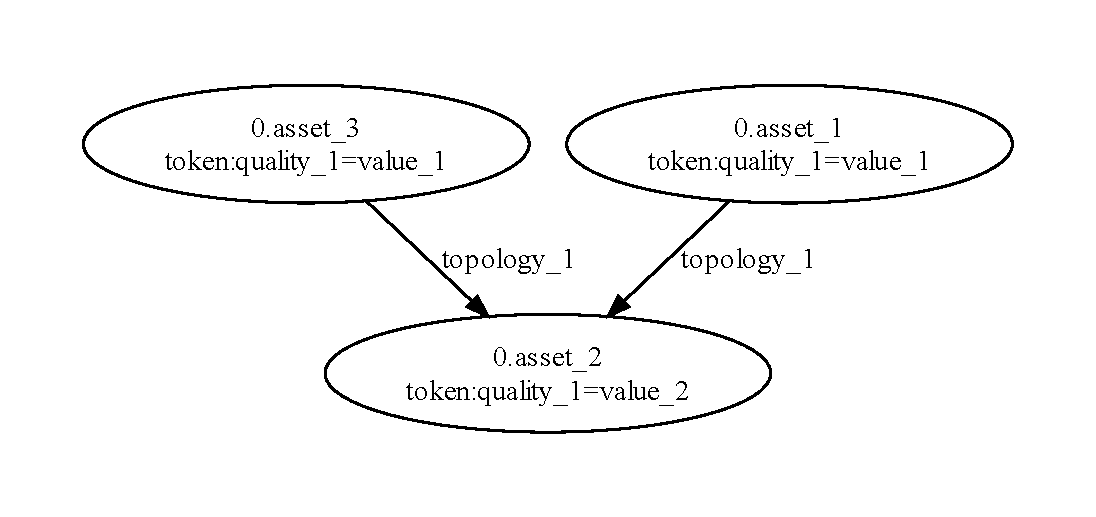
\includegraphics[width=4in]{ag_illustrative_simple/nm_state0}
\caption{State 0 of the illustrative discrete example}
\label{fig:ill_topology_0}
\end{figure}

Execution of the generation process begins by specifying a maximum ``depth''
of generation, which will be 2 for the purposes of this exercise, and by creating
an initial list of states for analysis, which contains only State 0.

Generation proceeds by examining each analysis state, in this case only State 0.
First, the generation function creates a list of all valid
attacks on State 0. Two such bindings are permitted: \texttt{exploit\_1 (asset\_1, asset\_2)},
and \texttt{exploit\_1 (asset\_3, asset\_2)}. Both bindings result in new states:
the first in State 1 (Fig.~\ref{fig:ill_topology_1}), and the second in State 2
(Fig.~\ref{fig:ill_topology_2}). Edges are added from State 0 to each as they are
generated. The current state of the attack graph is illustrated in 
Fig.~\ref{fig:ill_ag_depth1}. Both of these states are added to the
successor state list.

\begin{figure}
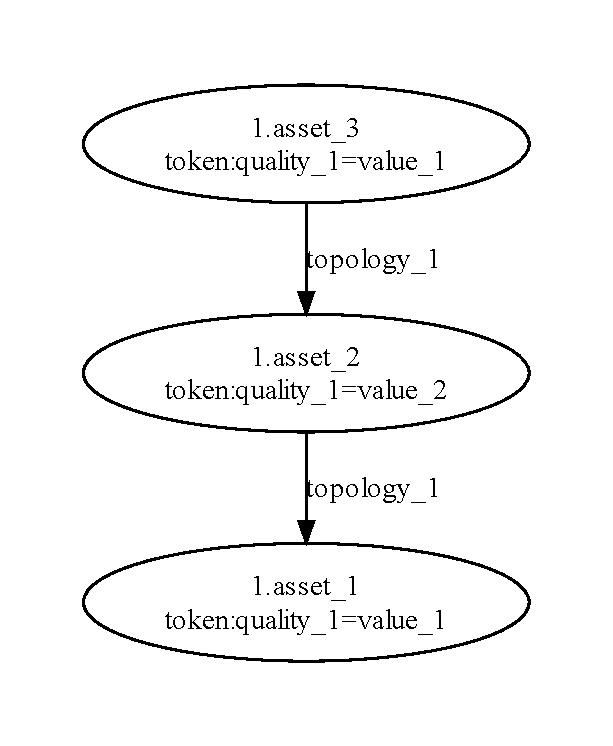
\includegraphics[width=4in]{ag_illustrative_simple/nm_state1}
\caption{State 1 of the illustrative discrete example}
\label{fig:ill_topology_1}
\end{figure}

\begin{figure}
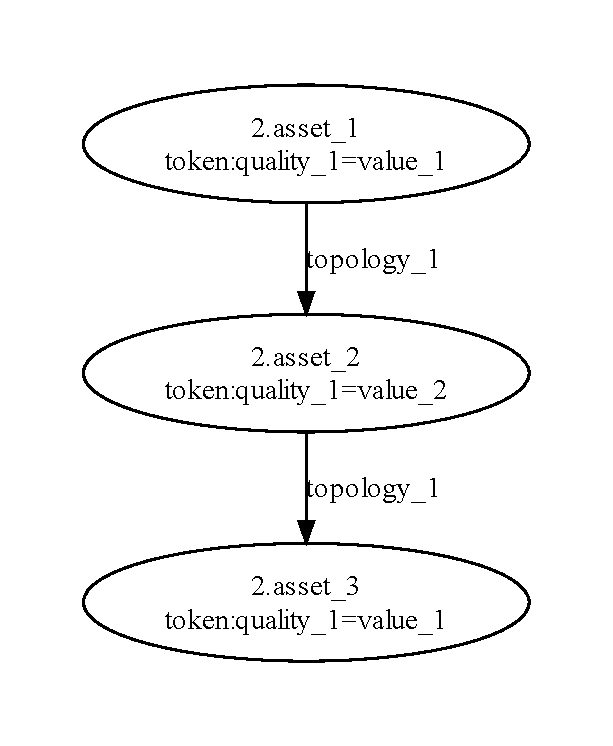
\includegraphics[width=4in]{ag_illustrative_simple/nm_state2}
\caption{State 2 of the illustrative discrete example}
\label{fig:ill_topology_2}
\end{figure}

\begin{figure}
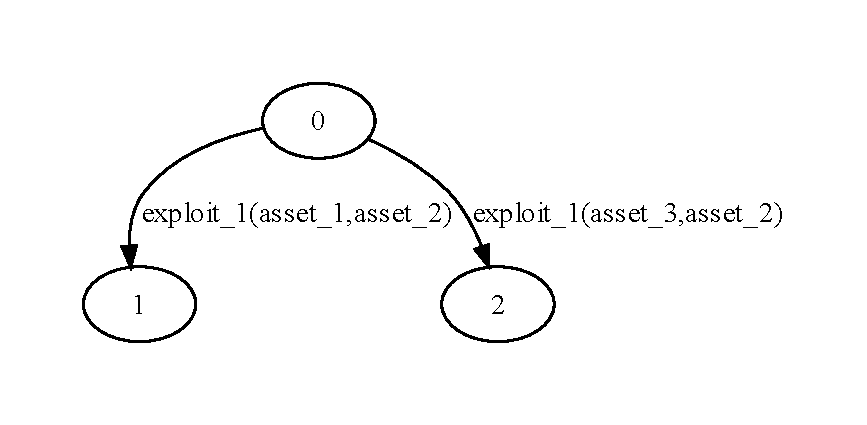
\includegraphics[width=4in]{ag_illustrative_simple/ag_depth1}
\caption{Attack graph after first iteration}
\label{fig:ill_ag_depth1}
\end{figure}

Remaining depth is reduced to 1, the successor state list becomes the
analysis state list, and generation proceeds again. In this case, the
analysis states are State 1 and State 2. Analysis begins with State 1. 
Two attacks are possible: \texttt{exploit\_1 (asset\_3, asset\_2)} and
\texttt{exploit\_2 (asset\_2, asset\_1)}. Both create new states, with the
former generating State 3 (Fig.~\ref{fig:ill_topology_3}) and the latter
generating State 4 (Fig.~\ref{fig:ill_topology_4}). Both of these are new
states, and they are added to the attack graph with the appropriate edges, as
well as to the successor state list.

\begin{figure}
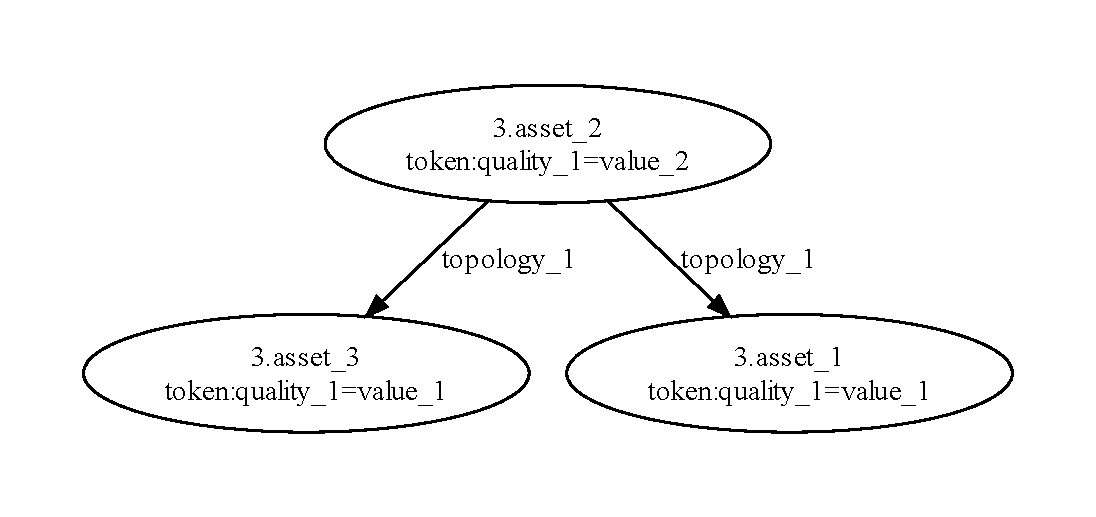
\includegraphics[width=4in]{ag_illustrative_simple/nm_state3}
\caption{State 3 of the illustrative discrete example}
\label{fig:ill_topology_3}
\end{figure}

\begin{figure}
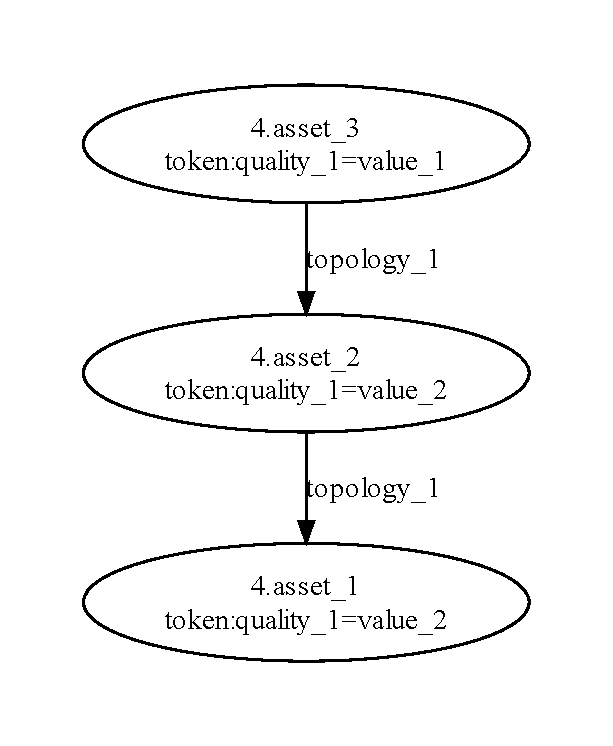
\includegraphics[width=4in]{ag_illustrative_simple/nm_state4}
\caption{State 4 of the illustrative discrete example}
\label{fig:ill_topology_4}
\end{figure}

Generation continues by addressing State 2. In State 2, two possible attacks
are returned: \texttt{exploit\_1 (asset\_1, asset\_2)} and 
\texttt{exploit\_2 (asset\_2, asset\_3)}. The first attack generates State 3,
an existing state. Since that state is already in the attack graph, it is
not added to the successor state list or to the attack graph again; instead,
only an edge is drawn. The second attack generates State 5 
(Fig.~\ref{fig:ill_topology_5}), which is new and is added to the attack graph
and the successor state list.

\begin{figure}
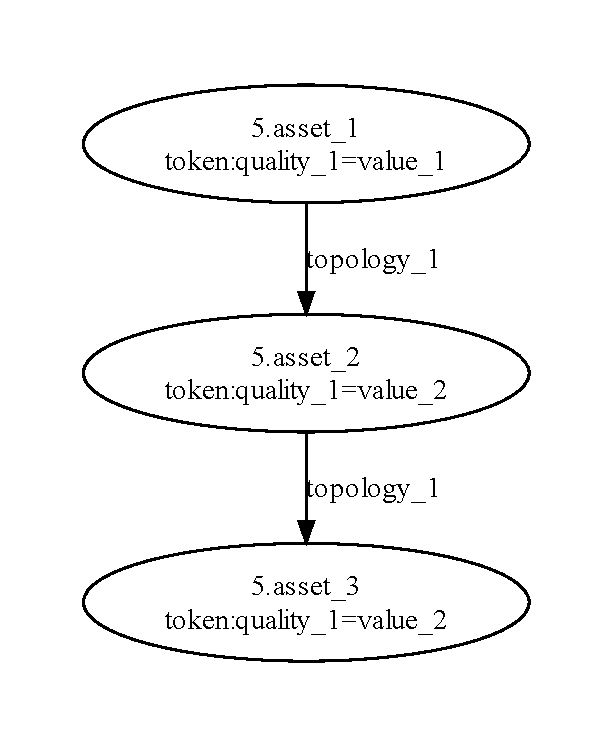
\includegraphics[width=4in]{ag_illustrative_simple/nm_state5}
\caption{State 5 of the illustrative discrete example}
\label{fig:ill_topology_5}
\end{figure}

For the next invocation, the successor state list becomes the analysis state
list, and the depth is reduced to 0.  Although there are more successor states,
the depth limit has been reached. Therefore, generation halts. The final product
attack graph is illustrated in Fig.~\ref{fig:ill_ag_depth2}. Incidentally, if
execution had been allowed to continue until there were no more successor states,
the generated attack graph would be the one in Fig.~\ref{fig:ill_ag_depth5}.

\begin{figure}
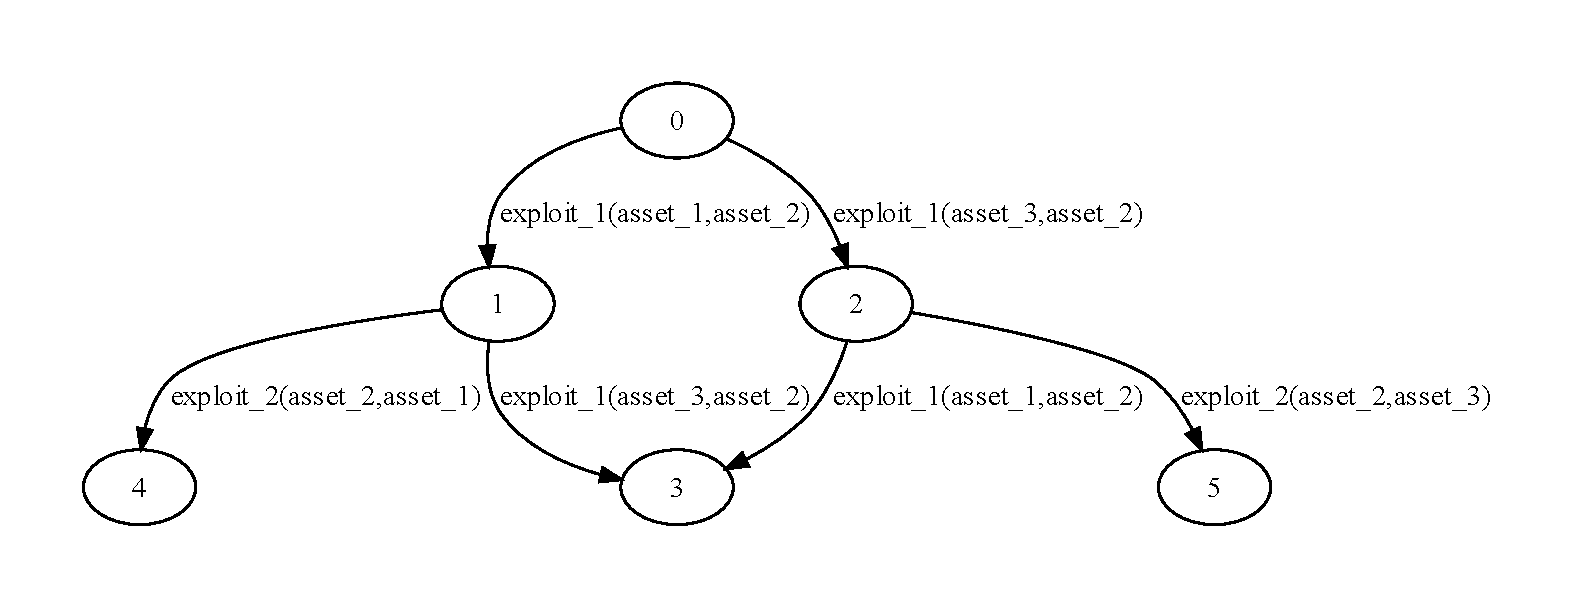
\includegraphics[width=4in]{ag_illustrative_simple/ag_depth2}
\caption{Attack graph after first iteration}
\label{fig:ill_ag_depth2}
\end{figure}

\begin{figure}
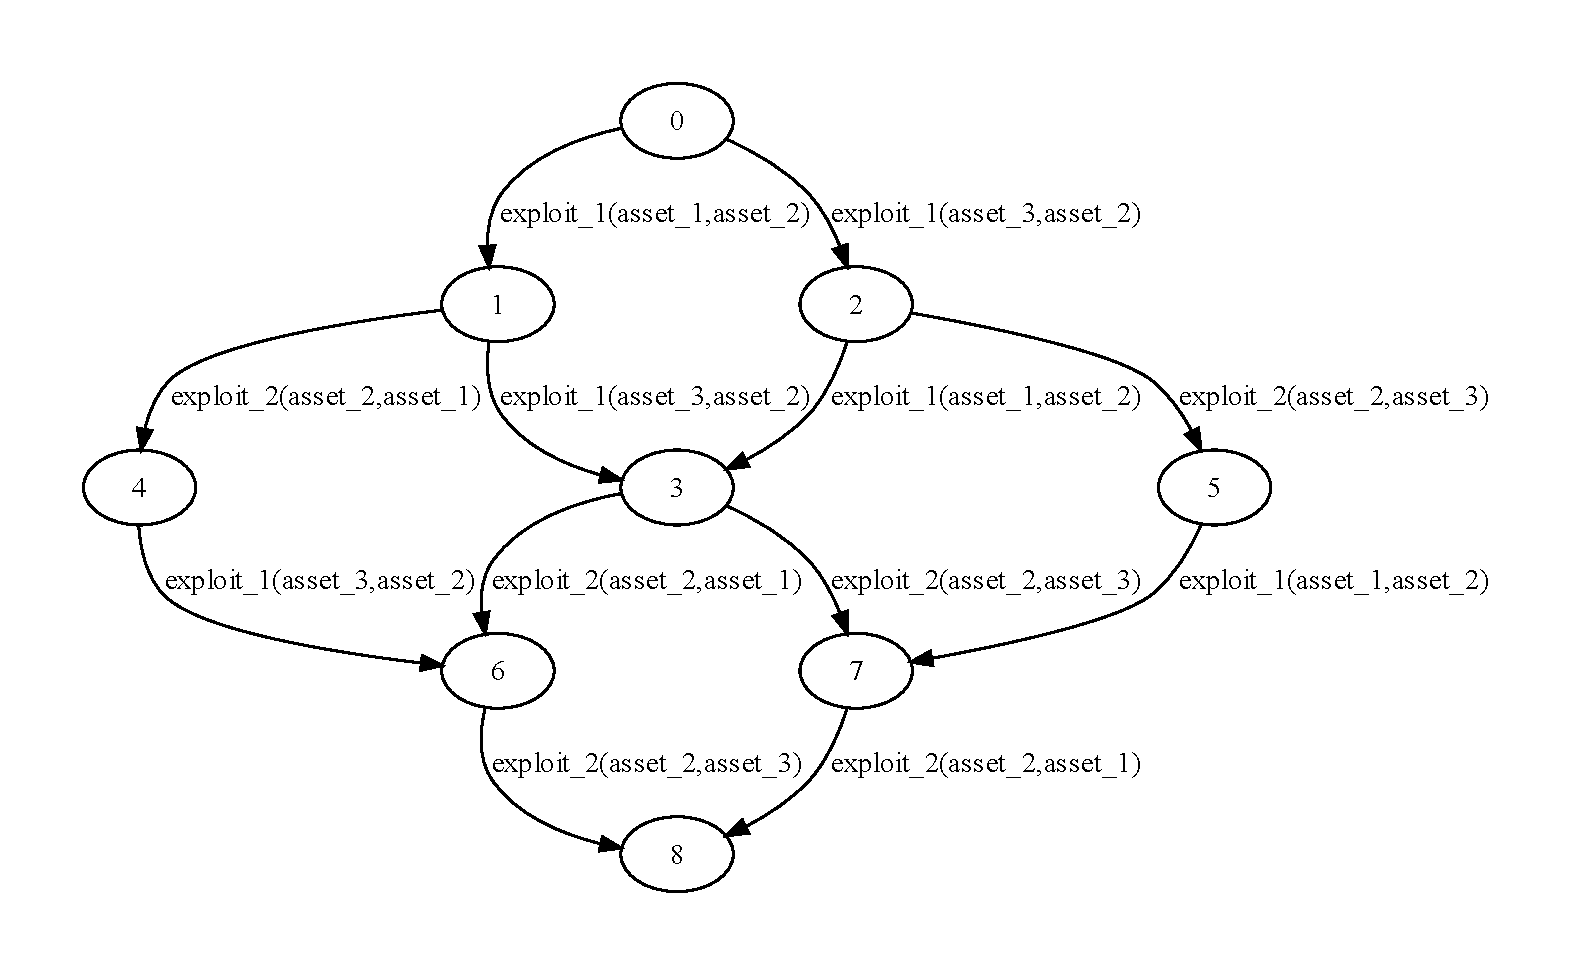
\includegraphics[width=4in]{ag_illustrative_simple/ag_depth5}
\caption{Complete illustrative attack graph}
\label{fig:ill_ag_depth5}
\end{figure}

This concludes the description of the basic attack graph modeling framework 
employed at 
the University of Tulsa. The chapters following this one are devoted to
this framework's expansion and analysis.